\documentclass[11pt]{article}

% American letter size:
\textwidth6.5in \textheight9in \oddsidemargin 0pt \evensidemargin 0pt
\topmargin -47pt


\usepackage{times}
\usepackage{fullpage}
\usepackage{epic}
\usepackage{subfigure}
\usepackage{eepic}
\usepackage{epsfig}
\usepackage{color}
\usepackage{amsmath,amsthm,amssymb}
\usepackage{amsfonts}
\usepackage{float}
\usepackage{appendix}
\usepackage{multirow}
\usepackage{booktabs}
\usepackage{url}

\renewcommand\floatpagefraction{1.0}
\renewcommand\topfraction{1.0}
\renewcommand\bottomfraction{0.9}
\renewcommand\bottomfraction{1.0}
\renewcommand\textfraction{0.0}

\newenvironment{enum*}%
 {\begin{enumerate}%
   \setlength{\itemsep}{-5pt}%
   \setlength{\parsep}{-5pt}%
   \setlength{\topsep}{-5pt}}%
 {\end{enumerate}}

\newenvironment{item*}%
 {\begin{itemize}%
   \setlength{\itemsep}{-5pt}%
   \setlength{\parsep}{-5pt}%
   \setlength{\topsep}{-5pt}}%
 {\end{itemize}}

\newcommand{\tup}[1]{%
        \relax\ifmmode
	           \langle #1 \rangle%
        \else
                $\langle$#1$\rangle$%
        \fi
}

\theoremstyle{plain}
\floatstyle{ruled}
\newfloat{algo}{htbp}{algo}
\floatname{algo}{Algorithm}
\usepackage[noend]{algorithmic}
\usepackage{distribalgo}

%\usepackage{setspace}
%\doublespacing

\newtheorem{thm}{Theorem}
\newtheorem{lemma}{Lemma}
\newtheorem{claim}{Claim}
\newtheorem{corollary}{Corollary}
\newtheorem{definition}{Definition}
\newtheorem{property}{Property}
\newtheorem{proposition}{Proposition}
\newtheorem{observation}{Observation}
\newtheorem{conjecture}{Conjecture}
\newtheorem{designrule}{Design Principle}
\newtheorem{invariant}{Invariant}
\newtheorem{theorem}{Theorem}

\newcommand{\up}[1]{\ensuremath{^{\textrm{#1}}}}
\newcommand{\down}[1]{\ensuremath{_{\textrm{#1}}}}
\newcommand{\tb}{\makebox[0.6cm]{}}
\newcommand{\negspace}{\vspace{-0.6\baselineskip}}
\newcommand{\snegspace}{\vspace{-0.25\baselineskip}}
\def\hyph{-\penalty0\hskip0pt\relax}

\newenvironment{restate}[1]{\begin{trivlist} \item {\bf #1 (restated)} \em}
  {\end{trivlist}}

\definecolor{Gray}{rgb}{0.1,0.4,0.1}
\definecolor{DarkBlue}{rgb}{0.2,0.2,0.5}
\definecolor{Cyan}{rgb}{0.5,0.2,0.5}
\newcommand{\comment}[1]{{\color{Gray}{$\rhd$ #1}}}
\newcommand{\elcomment}[1]{\hfill{\comment{#1}}}
\newcommand{\funcname}[1]{\textsc{\color{DarkBlue}{#1}}}
\newcommand{\typename}[1]{\textbf{\color{Cyan}{#1}}}

%\setlength\topmargin{-0.025in}
%\setlength\textheight{8.75in}

%%=======================================================================
%% Latex template for SPAA 2012
%%=======================================================================
%
%% remember to compile with dvips -t letter for US letter style
%
%\documentclass[11pt]{article}
%
%% American letter size:
%\textwidth6.5in \textheight9in \oddsidemargin 0pt \evensidemargin 0pt
%\topmargin -47pt
%
%\usepackage{times}
%
%\newtheorem{theorem}{Theorem}[section]
%\newtheorem{lemma}[theorem]{Lemma}
%\newtheorem{claim}[theorem]{Claim}
%\newtheorem{fact}[theorem]{Fact}
%
%\newcommand{\sq}{\hbox{\rlap{$\sqcap$}$\sqcup$}}
%\newcommand{\qed}{\hspace*{\fill}\sq}
%\newenvironment{proof}{\noindent {\bf Proof.}\ }{\qed\par\vskip 4mm\par}
%\newenvironment{proofof}[1]{\bigskip \noindent {\bf Proof of #1:}\quad }
%{\qed\par\vskip 4mm\par}



\begin{document}

\begin{titlepage}

\title{A Low Synchronization NUMA-aware Algorithm for Producer-Consumer Pools \\
       {\Large (Regular Submission)}}

\author{Elad Gidron \\
   eladgi@cs.technion.ac.il \\
   \and
   Idit Keidar \\
   idish@ee.technion.ac.il \\
   \and
   Dmitri Perelman \\
   dima39@tx.technion.ac.il \\
   \and
   Yonathan Perez \\
   yonathan0210@gmail.com
   } 

\date{Department of Electrical Engineering, Technion, Haifa, Israel}

\maketitle \thispagestyle{empty}

\begin{abstract}
We present a non-blocking starvation-free producer-consumer task pool, designed with a special emphasis on lightweight synchronization and data locality.
The core building block of our pool is SALSA, Scalable And Low Synchronization Algorithm for a single-consumer container with the task stealing support. Each consumer operates its own SALSA container, stealing the tasks from other containers if necessary. An elegant self-stabilizing policy for task insertion does not push tasks to the overloaded SALSA containers, thus decreasing the possibility of stealing transactions. 

SALSA organizes tasks in large chunks improving locality properties and simplifying the stealing. The use of page-size chunks perfectly suits the data migration schemes among the processor nodes available in NUMA architectures. 
Thanks to the novel approach for coordination among consumers, our system does not use strong atomic operations or memory barriers in the fast path and invokes only a single CAS operation during the chunk steal. 

The evaluation experiments demonstrate that the pool built upon SALSA containers scales linearly with the number of threads and significantly outperforms other non-FIFO alternatives.

\end{abstract}

\bigskip

\centerline{{\bf Keywords}: multi-core, concurrent data structures.}

\end{titlepage}

\section{Introduction}
\label{sec:intro}

\section{Related Work}
\label{sec:related}
\paragraph{Task pools.}
There is a large body of work on lock-free unbounded FIFO queues and LIFO
stacks~\cite{Gidenstam:2010:CLQ:1940234.1940266,Hendler:2004:SLS:1007912.1007944,
Hoffman:2007:BQ:1782394.1782423, Michael:1996:SFP:248052.248106,Moir:2005:UEI:1073970.1074013}.
The problem with such algorithms is that due to the inherent need for ordering all operations, they
generally have high contention and hence do not scale well being therefore less appealing for use as 
consumer-producer task pools. 

A number of previous works have recognized this limitation, and observed that strict FIFO
order is seldom needed in multi-core systems~\cite{Afek:2010:SPP:1885276.1885295,springerlink:10.1007/978-3-642-17653-1_29,
Basin:2011:CST:2075029.2075087,Sundell:2011:LAC:1989493.1989550}. However, all of these solutions
use strong atomic operations, at least in every consume operation. Most of
them~\cite{Afek:2010:SPP:1885276.1885295,springerlink:10.1007/978-3-642-17653-1_29,
Basin:2011:CST:2075029.2075087} do not partition the pool among chips, and therefore do not achieve
good locality and cache-friendliness, which limits their scalability on NUMA systems~\cite{Basin:Thesis:2011}.

The non-FIFO pool that is closest to our work is the Concurrent Bags of
Sundell et al.~\cite{Sundell:2011:LAC:1989493.1989550}, which, like SALSA, is composed of
per-producer chunk lists. Unlike our pool, however, their algorithm uses strong atomic operations
upon each consume. In addition, steals are performed in the granularity of single tasks and
not whole chunks as in SALSA. Overall, Concurrent Bags throughput does not scale linearly with the number of participating threads.

\paragraph{Techniques.}
Variations of techniques we employ were previously used in various contexts. 
Work-stealing~\cite{Blumofe:1999:SMC:324133.324234} is a standard way to reduce
contention by using individual per-consumer pools, where tasks may be stolen from one pool to
another. 
Partitioning of tasks into per-consumer pools also allows optimizing performance in the
case where a consumer is working on its own pool without being interrupted by stealing; we refer to
this case as the \emph{fast-path}. The concept of a synchronization-free fast-path previously
appeared in works on scheduling queues,
e.g.,~\cite{Arora:1998:TSM:277651.277678,Hendler:2006:DNW:1160290.1160294}. However, these works
assume that the same process is both the producer and the consumer, and hence the
synchronization-free fast-path is actually used only when a process transfers data to \emph{itself}.
On the other hand, our pool is synchronization-free even when tasks are transfered among multiple
threads; our synchronization-free fast-path is used also when multiple producers produce data for
a single consumer. We do not know of any other work that supports synchronization-free data
transfer among different threads.

We improve the efficiency of stealing by transferring a chunk of tasks upon every steal
operation. Hendler et al.~\cite{Hendler:2002:NSW:571825.571876} have proposed stealing of multiple
items by copying a range of tasks from one dequeue to another. Unfortunately, this approach requires
costly CAS operations on the fast-path and introduces non-negligible overhead for item copying. In
contrast, our approach of chunk-based stealing coincides with our synchronization-free fast-path,
and steals whole chunks in O(1) steps. Furthermore, our use of page-size chunks allows for data
migration in NUMA architectures to improve locality.

Finally, the technique of organizing data in chunks allows building dynamically sized data
structures while preserving data locality. Chunk-based data structures were previously used
in~\cite{Braginsky:2011:LLL:1946143.1946153, Gidenstam:2010:CLQ:1940234.1940266,
Hendler:2006:DNW:1160290.1160294, Sundell:2011:LAC:1989493.1989550}. SALSA extends on the idea of
using chunk-based data structures by using chunks also for efficient stealing.

\section{System Overview}
\label{sec:system}
In the current section we present our framework for scalable and NUMA-aware producer-consumer data exchange. 
Our system follows the principle of separating mechanism and policy.
To this end, we consider two independent logical entities: 
\begin{enumerate}
	\item \emph{A single consumer pool (SCPool)} mechanism manages the tasks arriving to a given consumer while introducing the possibility of stealing some tasks by other consumers.
	\item A management policy is responsible for operating SCPools: the policy routes producers' requests to the appropriate consumers and initiates stealing between the pools. This way, the policy controls the system's behavior according to considerations of load-distribution, throughput, fairness, locality, etc.
	We are especially interested in a management policy suitable for Non-Uniform Memory Access (NUMA) architectures (see Figure~\ref{fig:system-fig}), where each CPU has its own memory, and accessing the memory of other CPUs is executed over an interconnect. As a high rate of remote memory accesses can decrease the overall performance, it is highly desirable for an SCPool of a consumer to reside at the RAM close to its own CPU. 
\end{enumerate} 

\paragraph{SCPool abstraction.}
\begin{algo}[!ht]
\caption{API for a Single Consumer Pool with stealing support.} 
\label{alg:scpool-api}
\begin{distribalgo}[1]
\scriptsize

\INDENT {\bf SCPool API:}
	\STATE produce(Task) \elcomment {Insert the task to the pool, returns false if no space left in the pool.}
	\STATE produceForce(Task) \elcomment {Inserts the task to the pool, expanding the pool if necessary. }
	\STATE consume() \elcomment {Retrieves a task from the pool, returns $\bot$ if no tasks in the pool are detected.}
	%\STATE getStealingScore() \elcomment {Returns a score corresponding to the amount of tasks to steal.}
	\STATE steal(SCPool from) \elcomment{Tries to steal a number of tasks from the given pool and move them to the current pool. Returns one of the stolen tasks or $\bot$. }%We guarantee that if there are tasks in the \emph{from} pool at the beginning of steal invocation, then either steal function returns a task, or there is another thread that returns a task during the steal execution.}
\ENDINDENT

\end{distribalgo}
\end{algo}

The SCPool API provides the abstraction of a single-consumer task pool with stealing support, see Algorithm~\ref{alg:scpool-api}.
A producer can invoke two types of insertion operations: \emph{produce}, which attempts to insert a task to the given pool and fails if the pool is full, and \emph{produceForce}, which always succeeds by expanding the pool on demand.
There are also two ways to retrieve a task from the pool: the owner of the pool (only) can call the \emph{consume} function; while any other thread can invoke the \emph{steal} function, which tries to transfer a number of tasks between the pools and return one of the stolen tasks. 
The pool must guarantee the following \emph{stealing property}, which is necessary for system liveness:
\begin{property}
If an SCPool is not empty at the beginning of a steal operation, then either the steal operation retrieves a task, or another thread retrieves a task during the steal execution.
\end{property}

A straightforward way to implement the API described above is to use a dynamic-size multi-producer multi-consumer FIFO queue (e.g., Michael-Scott queue~\cite{Michael:1996:SFP:248052.248106}).
In this case, both produce() and produceForce() enqueue a new task, while both consume() and steal() dequeue a task. In the next section we present SALSA, a much more efficient SCPool.

\begin{figure}[htb]
	\centering
	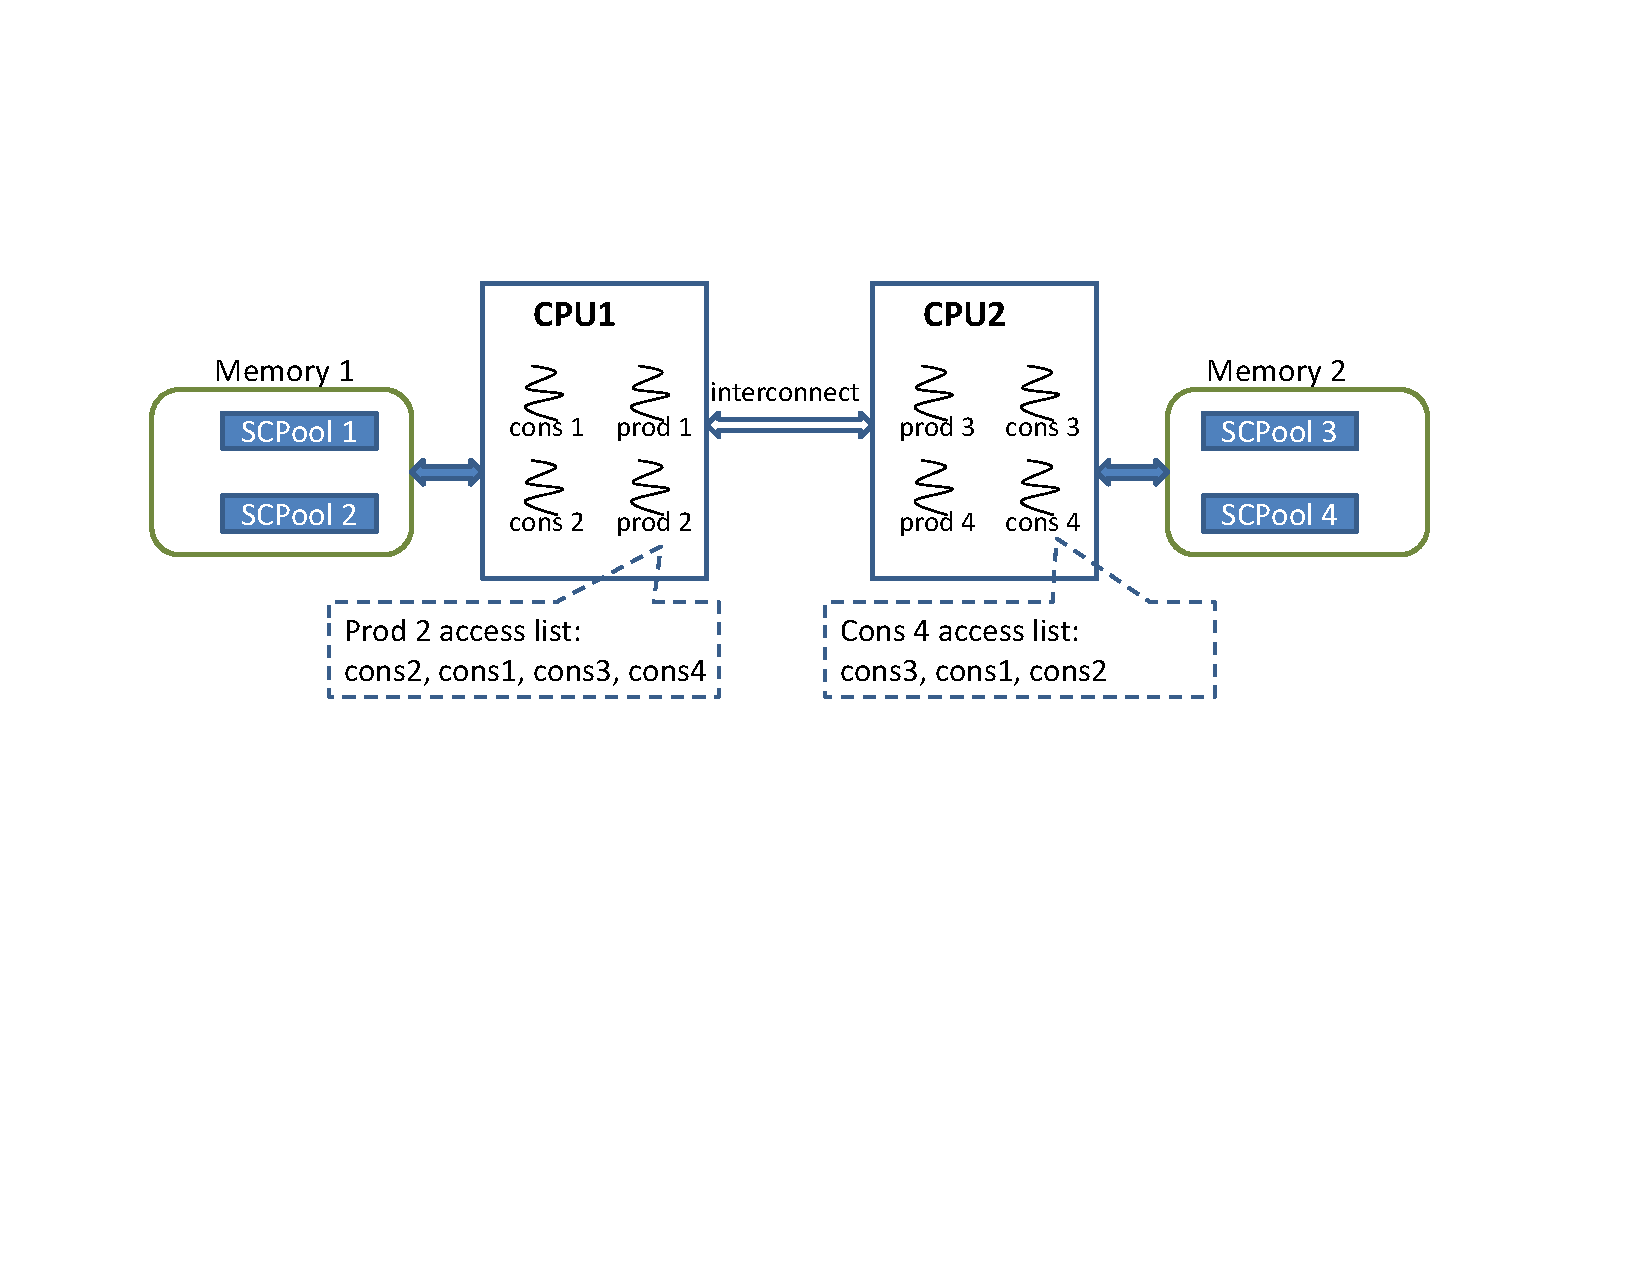
\includegraphics[width=0.7\textwidth]{figures/system-fig}
	\caption{\footnotesize{System overview of the management framework. In the given example the system is composed of two processors that are connected to their own memory banks (NUMA architecture). There are two producers and two consumers running on each processor, the data of each consumer is allocated at the closest available physical memory. A producer $p_i$ has an access list of consumers for task insertion. A consumer $c_i$ has an access list of consumers for task stealing. }}
	\label{fig:system-fig}
\end{figure}

\paragraph {Management policy.}
A management policy is generally defined by the way in which: (1) a producer chooses one of the SCPools to insert a task to, and when it chooses to use produce force; and (2) a consumer decides when to retrieve a task from its own pool and steal tasks from other pools. 
Note that the policy is independent of the underlying SCPool implementation. We believe that it is a subject for engineering optimizations, based on specific workloads and demands.


In the current work, we present a policy that exploits the locality properties of NUMA architectures and is aimed at achieving maximal throughput. If the individual SCPools themselves are lock-free and starvation-free, then our policy preserves these properties at the system level. Our policy is as follows:
\begin{itemize}
	\item {\bf Access lists.} Each process in the system (producer or consumer) is provided with an \emph{access list}, an ordered list of consumers, sorted according to their distance from that process (see Figure~\ref{fig:system-fig}). Intuitively, our policy is to have a producer mostly interact with the closest consumer, while stealing mainly happens inside the same processor node. 
	\item {\bf Producer's policy.} A producer inserting a task first calls the \emph{produce} function of the first SCPool in its access list. Note that a produce operation might fail if the pool is full, (which can be seen as evidence of that the corresponding consumer is overloaded).  In this case, the producer tries to insert the task into other pools, in the order defined by its access list. If all insertions fail, the producer invokes the \emph{produceForce} operation on the closest SCPool, which always succeeds (expanding the pool if needed). 
	\item {\bf Consumer's policy.} A consumer consumes tasks from its own SCPool. If its SCPool is empty, the consumer tries to steal tasks from other pools in the order defined by its access list. 
\end{itemize}



% The inter-pool communication policy is a subject to engineering optimizations and its optimal behavior should probably
% depend on the workload. For the purpose of our evaluation we propose the following approach. 
	% Producer policy. Each producer is provided with the list of all available consumers sorted according to the locality considerations of the given architectures. For example, in case of 
% In order to insert a task a producer first invokes a produce() operation on the closest consumer. If this operation fails, 
% then the closest consumer's pool is full (which could be evidence of an over-load of the given consumer thread) and the producer should 
% try to insert a task to another consumer. If neither consumer ... a producer finally invokes produceForce(), which expands the pool if necessary and always succeeds to insert the task. 
	% Consumer policy. A consumer works in a loop of consuming its own tasks. If the own pool of a consumer is empty, the consumer iterates over all other consumers and tries to steal tasks from there. 




\section{Algorithm Description}
\label{sec:algo}
\newcounter{alg:non-fifo:lines}
\begin{algo}[!ht]
\caption{Non-FIFO implementation of SCPool: Data Structures.} 
\label{alg:non-fifo-ds}
\scriptsize
\begin{minipage}[t]{0.48\textwidth}
\begin{distribalgo}[1]
\smallskip

\INDENT {{\bf Chunk data structure}:}
	\STATE Task[CHUNK\_SIZE] tasks 
  \STATE int owner \comment {owner's consumer id}
\ENDINDENT

\INDENT {{\bf Node data structure}:}
  \STATE Chunk c; initially $\bot$
  \STATE int idx; initially -1
\ENDINDENT

\setcounter{alg:non-fifo:lines}{\value{ALC@line}} % store the line number
\end{distribalgo}
\end{minipage}%
%
\hfill
%
\begin{minipage}[t]{0.48\textwidth}
%
\begin{distribalgo}[1]
\setcounter{ALC@line}{\value{alg:non-fifo:lines}}
\smallskip

\INDENT {{\bf SCPool per consumer data structure}:}
  \STATE int consumerId
  \STATE List\tup{Node}[] chunkLists \comment {one list per producer + extra list for stealing (single-writer multi-reader)} 
  \STATE ChunkPool chunkPool \comment {the pool of spare chunks}
  \STATE Node currentNode, initially $\bot$ \comment {current node to work with} 
\ENDINDENT

\setcounter{alg:non-fifo:lines}{\value{ALC@line}}
\end{distribalgo}
\end{minipage}
\end{algo}

\begin{algo}[!ht]
\caption{Non-FIFO implementation of SCPool: Producer Functions.}
\label{alg:producer-non-fifo}
\scriptsize
\begin{minipage}[t]{0.48\textwidth}
\begin{distribalgo}[1]
\setcounter{ALC@line}{\value{alg:non-fifo:lines}}

\INDENT {{\bf Producer local variables}:}
	\STATE int producerId
	\STATE Chunk chunk; initially $\bot$ \comment {the chunk to insert to}
	\STATE int prodIdx; initially $0$ \comment {the prefix of inserted tasks}
\ENDINDENT

\setcounter{alg:non-fifo:lines}{\value{ALC@line}} % store the line number
\end{distribalgo}
\end{minipage}%
%
\hfill
%
\begin{minipage}[t]{0.48\textwidth}
%
\begin{distribalgo}[1]
\setcounter{ALC@line}{\value{alg:non-fifo:lines}}

\INDENT {{\bf Function produce}(Task t, SCPool scPool):}
	\INDENT {{\bf if} (chunk $= \bot$) {\bf then}}
		\STATE newChunk $\leftarrow$ a chunk from scPool.chunkPool
		\STATE {\bf if} (chunk $= \bot$) {\bf then return FULL} \comment {no available chunks}
		\STATE newChunk.owner $\leftarrow$ scPool.consumerId
		\STATE node $\leftarrow$ new node with idx $=-1$ and c $=$ newChunk
		
		\STATE scPool.chunkLists[producerId].{\bf append}(node)
		\STATE chunk $\leftarrow$ newChunk; prodIdx $\leftarrow 0$ 
	\ENDINDENT
	\STATE chunk.tasks[prodIdx] $\leftarrow$ t; prodIdx++
	\INDENT {{\bf if}(prodIdx $=$ CHUNK\_SIZE) {\bf then}}
	  \STATE chunk $\leftarrow \bot$ \comment {the chunk is full}
	\ENDINDENT
	\STATE {\bf return SUCCESS}
\ENDINDENT

\setcounter{alg:non-fifo:lines}{\value{ALC@line}}
\end{distribalgo}
\end{minipage}
\end{algo}

\begin{algo}[!ht]
\caption{Non-FIFO implementation of SCPool: Consumer Functions.} 
\label{alg:non-fifo}
\scriptsize
\begin{minipage}[t]{0.48\textwidth}
\begin{distribalgo}[1]
\setcounter{ALC@line}{\value{alg:non-fifo:lines}}
\smallskip


\INDENT {{\bf Function consume}():}
  \INDENT {{\bf if}(currentNode $\neq \bot$) {\bf then} \comment {common case}}
		\STATE t $\leftarrow$ {\bf takeTask}(currentNode)
		\STATE {\bf if} (t $\neq \bot$) {\bf then return} t
	\ENDINDENT
	\comment {Iterate over other chunk lists}
	\INDENT {{\bf foreach} cl {\bf in} chunkLists {\bf do} \comment {fair traversal}} 
  	\INDENT {{\bf foreach} node {\bf in} cl {\bf do}}
  		\STATE t $\leftarrow$ {\bf takeTask}(node)
			\STATE {\bf if} (t $\neq \bot$) {\bf then} currentNode $\leftarrow$ node; {\bf return} t
  	\ENDINDENT
	\ENDINDENT
	\STATE currentNode $\leftarrow \bot$; {\bf return} $\bot$
\ENDINDENT

\medskip

\INDENT {{\bf Function takeTask}(Node n):}
  \STATE chunk $\leftarrow$ n.c
  \STATE {{\bf if} (chunk $= \bot$) {\bf then return $\bot$} \comment{this chunk has been stolen}}
 
  \STATE task $\leftarrow$ chunk.tasks[n.idx + 1]
  \STATE {\bf if} (task $= \bot$) {\bf then return} $\bot$ \comment{no inserted tasks}
 	
 	\smallskip 
  \STATE n.idx++ \comment {tell the world you're going to take a task from idx}
  \INDENT {{\bf if} (chunk.owner $=$ consumerId) {\bf then} \comment {common case}}
 		\STATE chunk.tasks[n.idx] $\leftarrow$ TAKEN
  	\INDENT {{\bf if}(n.idx + 1 $=$ CHUNK\_SIZE) {\bf then} \comment {finished the chunk}}
  		\STATE n.c $\leftarrow \bot$; return the chunk to the chunkPool
  		\STATE currentNode $\leftarrow \bot$
  	\ENDINDENT
  	\STATE {\bf return} task 
  \ENDINDENT
  
  \smallskip
  \comment {the chunk has been stolen, CAS the last task and go away}
 	\STATE success $\leftarrow$ (task $\neq$ TAKEN $\wedge$ \\
 		\hspace{0.5cm} CAS(chunk.tasks[n.idx], task, TAKEN))
	\STATE n.c $\leftarrow \bot$; currentNode $\leftarrow \bot$
 	\STATE {\bf return} (success) ? task : $\bot$
\ENDINDENT

\setcounter{alg:non-fifo:lines}{\value{ALC@line}} % store the line number
\end{distribalgo}
\end{minipage}%
%
\hfill
%
\begin{minipage}[t]{0.48\textwidth}
%
\begin{distribalgo}[1]
\setcounter{ALC@line}{\value{alg:non-fifo:lines}}
\smallskip

\INDENT {{\bf Function steal}(SCPool from):}
	\STATE prevNode $\leftarrow$ a node holding tasks from some list \comment {different policies possible}
	\STATE c $\leftarrow$ prevNode.c;
  \STATE {\bf if} (c = $\bot$) {\bf then return} $\bot$

	\comment {add prevNode to steal list to make it re-stealable}
  \STATE chunkLists[steal].{\bf append}(prevNode)
  \INDENT {{\bf if} ({\bf CAS}(c.owner, from.consumerId, consumerId) $=$ false)}
 		\STATE chunkLists[steal].{\bf remove}(prevNode)
 		\STATE {\bf return} $\bot$ \comment {failed to steal}
	\ENDINDENT
	\STATE {\bf if}(prevNode.idx $+1$) {\bf then}
	\smallskip
	\STATE newNode $\leftarrow$ copy of prevNode
	\STATE replace prevNode with newNode in chunkLists[steal]
	\STATE prevNode.c $\leftarrow \bot$ \comment {done stealing the chunk, take its task}
	
	\smallskip
	\STATE idx $\leftarrow$ newNode.idx
	\STATE task $\leftarrow$ c.tasks[idx+1] 
	\STATE {\bf if} (task $= \bot$) {\bf then return} $\bot$ \comment {still no task at idx+1}
	\INDENT {{\bf if} (task $=$ TAKEN $\vee$ \\
		\hspace{0.5cm} !CAS(c.tasks[idx+1], task, TAKEN)) {\bf then}} 
		\STATE task $\leftarrow \bot$
	\ENDINDENT
	\STATE currentNode $\leftarrow$ newNode
	\INDENT {{\bf if}(newNode.idx + 1 $=$ CHUNK\_SIZE) {\bf then}}
  	\STATE newNode.c $\leftarrow \bot$; return the chunk to the chunkPool
  	\STATE currentNode $\leftarrow \bot$
  \ENDINDENT
	\STATE newNode.idx $\leftarrow$ newNode.idx+1
	\STATE {\bf return} task
\ENDINDENT

\setcounter{alg:non-fifo:lines}{\value{ALC@line}}
\end{distribalgo}
\end{minipage}
\end{algo}

%\begin{algo}[!ht]
%\caption{Non-FIFO implementation of SCPool: Auxiliary Functions.} 
%\label{alg:non-fifo-aux}
%\scriptsize
%\begin{minipage}[t]{0.48\textwidth}
%\begin{distribalgo}[1]
%\setcounter{ALC@line}{\value{alg:non-fifo:lines}}
%\smallskip
%
%\INDENT {{\bf Function getStealingScore}():}
%	\comment {return the max of all the chunkCounters}
%	\STATE res $\leftarrow 0$
%	\INDENT {{\bf for} i $= 0, \ldots, $ NUM\_PRODUCERS {\bf do}}
%		\STATE {\bf if} (chunkCounters[i] $>$ res) res $\leftarrow$ chunkCounters[i]
%	\ENDINDENT
%	\STATE {\bf return} res
%\ENDINDENT
%
%\medskip
%\INDENT {{\bf Function isEmpty}(Node n):}
%  \STATE c $\leftarrow$ n.chunk
%  \STATE {\bf if} (c $= \bot$) {\bf then return true}
%  \STATE \comment {in empty chunk $\bot_2$ values are followed by $\bot$ values}
%  \INDENT {{\bf for} i $=$ n.idx, $\ldots$, i $<$ CHUNK\_SIZE {\bf do}}
%    \STATE {\bf if} (c.tasks[i] $= \bot$) {\bf then return true}
%    \STATE {\bf if} (c.tasks[i] $\neq \bot_2$) {\bf then return false} \comment {a task found}
%  \ENDINDENT
%  \STATE {\bf return true} \comment {no tasks found}
%\ENDINDENT
%
%\setcounter{alg:non-fifo:lines}{\value{ALC@line}} % store the line number
%\end{distribalgo}
%\end{minipage}%
%%
%\hfill
%%
%\begin{minipage}[t]{0.48\textwidth}
%%
%\begin{distribalgo}[1]
%\setcounter{ALC@line}{\value{alg:non-fifo:lines}}
%\smallskip
%\INDENT {{\bf Function chooseEntryForSteal}(SCPool from):}
%	\STATE maxNumChunks $\leftarrow 0$
%	\INDENT {{\bf for} i $= 0, \ldots, $ NUM\_PRODUCERS {\bf do}}
%		\INDENT {{\bf if} (from.chunkCounters[i] $>$ maxNumChunks) {\bf then}}
%			\STATE maxNumChunks $\leftarrow$ from.chunkCounters[i]
%			\STATE entryForSteal $\leftarrow$ i
%		\ENDINDENT
%	\ENDINDENT
%	\STATE {\bf return} entryForSteal
%\ENDINDENT
%
%\medskip
%
%\INDENT {{\bf Function removeNode}(Node n):}
%	\STATE {\bf FetchAndAdd}(chunkCounters[currentEntry],-1)
%	\STATE prodEntries[currentEntry].{\bf remove}(n)
%	\STATE currentNode $\leftarrow \bot$
%\ENDINDENT 
%
%\medskip
%
%\INDENT {{\bf Function checkLast}(Node n, Chunk c):}
%	\STATE {\bf if}(n.idx $+1 \neq $ CHUNK\_SIZE) {\bf then return}
%	\STATE \comment {this thread took the last task --- reclaiming}
%  \STATE {\bf reclaimChunk}(c); {\bf removeNode}(n)
%\ENDINDENT
%
%\setcounter{alg:non-fifo:lines}{\value{ALC@line}}
%\end{distribalgo}
%\end{minipage}
%\end{algo}


\section{Evaluation}
\label{sec:evaluation}

\section{Conclusions}
\label{sec:conclusions}

\bibliographystyle{abbrv}
\bibliography{refs}

\end{document}